
\OriginalPage{198}{}
\thispagestyle{empty}
\setcounter{chapter}{7}
\setcounter{section}{0}
\setcounter{figure}{0}
\noindent{\LARGE\bfseries 7.\quad A Simulation Environment\par}
\label{chap:simulation-environment}
\section{Introduction}
\label{sec:simenv-intro}

This chapter provides a user's view of a simulation environment called
SMPL. SMPL comprises the \texttt{smpl} simulation subsystem described in Chapter
2, additional debugging, analysis, and reporting tools, and an interactive
run-time interface called \texttt{mtr}. This description is based on an implementation
of SMPL called SMPL/PC, which runs on one type of personal computer.
Similar environments can be tailored to other systems; a design overview of
\texttt{mtr} and some of the SMPL tools is given in Chapter 9.

The SMPL simulation environment is illustrated in Figure 7.1. Basic
simulation operations are performed via simulation program calls to \texttt{smpl}
functions, as discussed in Chapter 2. \texttt{mtr} provides an interface between the
user, the simulation program, \texttt{smpl}, and other SMPL modules (most of these
also can be used directly from the simulation program). These modules
include the following.

\begin{description}
\item[\texttt{dump}.] This module displays the state (event list and queue
contents, facility users and status) of the simulated system.
This display can be invoked via \texttt{mtr} or by a simulation
program function call.
\item[\texttt{table}.] This module provides functions for table definition,
data entry, reporting, and plotting. These can be invoked via
\texttt{mtr} (for SMPL parameters) or by calls from the simulation
program.
\item[\texttt{bma}.] This is the batch means analysis module. A batch
means analysis is used to determine the simulation run
length required to achieve a specified accuracy for a model
output parameter. It can be initiated from \texttt{mtr} (for SMPL
parameters) or from the simulation program.
\end{description}

\OriginalPage{199}{7.1 Introduction}
\begin{figure}[H]
\centering
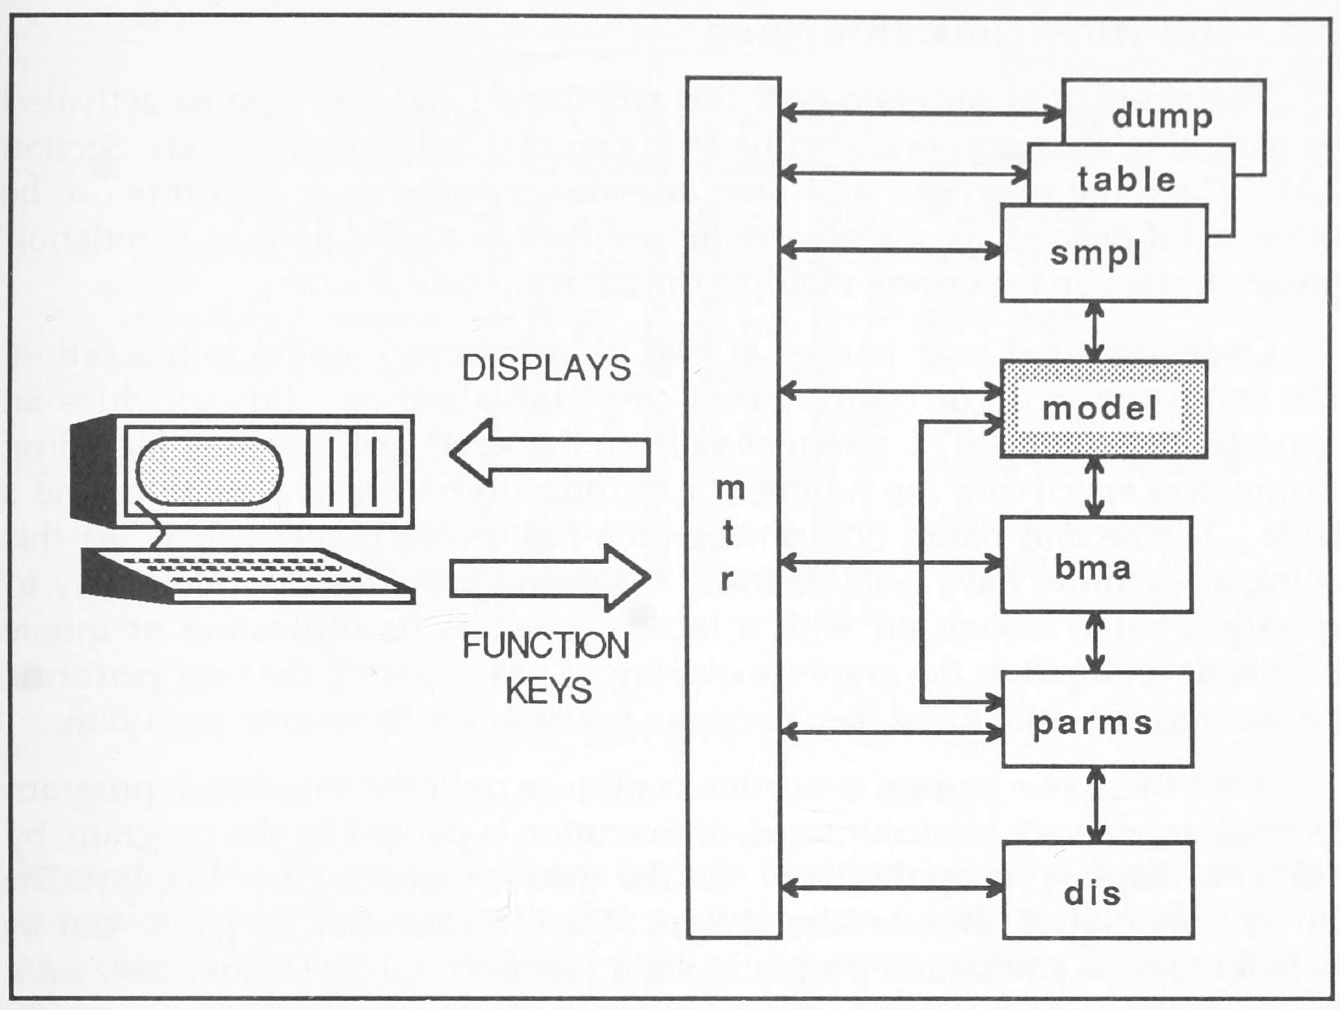
\includegraphics[width=\textwidth]{figures/ch7-figure-7-1.png}
\caption{The SMPL Simulation Environment}
\label{fig:smpl-environment}
\end{figure}

\begin{description}
\item[\texttt{parms}.] The \texttt{parms} module provides facilities for defining
and naming SMPL parameters. These are selected model
variables whose values can be assigned or displayed via \texttt{mtr}
as well as by the simulation program. They also can be designated
as inputs to table data entry, batch means analysis,
and graphics display functions.
\item[\texttt{dis}.] This module uses the computer's bit-mapped graphics
display to plot facility utilization, queue length, or a SMPL
parameter versus time, or to plot one SMPL parameter versus
another. This display can be initiated only from \texttt{mtr}.
\end{description}
Figure 7.1 provides a user-level view: lower-level SMPL modules, such as
the screen/keyboard services module, are not shown.

Subsequent sections describe \texttt{mtr}, SMPL parameters and the \texttt{parms} module,
and the \texttt{dump}, \texttt{table}, \texttt{bma}, and \texttt{dis} modules. These last four modules are
optional components of a SMPL system ``build''.


\OriginalPage{200}{A Simulation Environment}
\section{The Run-Time Interface}
\label{sec:simenv-mtr}

The simulation program specifies whether or not \texttt{mtr} is to be activated
by assigning the appropriate value to a \texttt{smpl()} call parameter (see Section
2.3). Thus, the overhead and user attendance associated with \texttt{mtr} can be
bypassed if desired, as when we're in ``production mode'' and the simulation
program is set up to perform multiple runs during one execution.

Once activated, \texttt{mtr} pauses at two points during model initialization.
The first pause occurs on completion of \texttt{smpl} initialization; this provides an
opportunity to set SMPL parameters from the keyboard, possibly including
parameters specifying the number of facilities to be defined, or to define a
table. The second pause occurs when the first event is scheduled. At this
point, all facilities have been defined; the pause provides an opportunity to
specify a value associated with a facility, such as its utilization or queue
length, as an input to the graphics display. At each pause, the user performs
the desired operations and then presses a function key to resume execution.

After these two pauses, execution continues until the simulation program
terminates, an error is encountered, or execution is paused by the program, by
a SMPL display, or by the user. As the model executes, \texttt{mtr} displays the
current simulation time on the screen. During execution, a pause can be
initiated by the simulation program, via a function call, or by the user, via a
function key. Also, SMPL modules typically initiate a \texttt{mtr} pause after
generating a display. If an error is detected by \texttt{smpl}, the error message is
displayed on the screen, and \texttt{mtr} pauses to permit the user to invoke the
\texttt{dump} and report displays (and possibly a simulation program display). The
simulation program usually displays the simulation report before terminating;
\texttt{mtr}, as a subprogram of \texttt{smpl}, terminates when the simulation program
terminates.

Monitoring operations are performed by a \texttt{mtr} function which is called by
\texttt{smpl} whenever an event occurs. This function checks to see if a breakpoint
match has occurred, updates any displays or analysis functions invoked from
\texttt{mtr}, and checks the keyboard to see if a function key has been pressed since
the last \texttt{mtr} entry (no other keys are recognized by \texttt{mtr} at this point).

The function key assignments of SMPL/PC are shown in Figure 7.2.\footnote{In this implementation, user-model interaction is based on function keys; other implementations may use pull-down (or pop-up) menus.}
The notes next to each key describe the key functions; the upper note indicates
the function executed when the key is pressed by itself, while the lower note
indicates the function executed when the key is pressed together with the
shift key. We'll refer to the normal functions keys as Fn, the shifted function

\OriginalPage{201}{7.2 The Run-Time Interface}
\begin{figure}[H]
\centering
\begin{tabular}{r c c l}
trace 1 toggle & F1 & F2 & trace 2 toggle \\
show help display & & & unassigned \\
trace 3 toggle & F3 & F4 & show report \\
show options & & & reset statistics \\
show output analysis & F5 & F6 & show dump \\
set up output analysis & & & set up graphics display \\
set breakpoint & F7 & F8 & set/show parameters \\
set random no.\ stream & & & invoke user display \\
show table or plot & F9 & F10 & pause/continue \\
set up table & & & print display \\
\end{tabular}
\caption{SMPL/PC Function Keys}
\label{fig:smpl-function-keys}
\end{figure}

\noindent keys as sFn. By using the appropriate function key, the user can pause
execution (or resume execution after a pause), turn tracing on and off, generate
any output display, invoke an initialization panel (screen display) for the
table, batch means, or graphics display functions, and display or modify
SMPL parameter values.

The F10 key is used to pause execution, resume execution after a pause,
and exit from displays. Pressing F10 while the simulation is running pauses
execution in a state called \emph{monitor pause} state. Any display may be invoked
from this state, and exit from displays is to this state. Pressing F10 while in
monitor pause state causes execution to be resumed. However, it is not
necessary to use F10 to pause execution prior to invoking a display; any
function key can be pressed at any time while the simulation is running.
Also, it is possible to invoke one display from another. As an example of
display sequencing, suppose the simulation is running and F6 is pressed. This
invokes the \texttt{dump} display, which may require stepping through several
panels. When the final panel is reached, the user can print the dump by
pressing sF10, exit to monitor pause state by pressing F10, or invoke another
display, such as the simulation report, by pressing the appropriate function
key.

Certain keys provide access to \texttt{smpl} functions. Keys F1--F3 turn \texttt{smpl}
tracing on and off. Trace 1 is free-running, trace 2 pauses after each full
screen, and trace 3 pauses after each trace message. These keys are toggles;
pressing a key once turns tracing on, pressing it again turns tracing off.

\OriginalPage{202}{A Simulation Environment}
\noindent Execution is resumed after a pause by pressing F10. The F4 key displays the
\texttt{smpl} simulation report which, depending on the number of facilities defined
in the model, may comprise more than one panel. When the final panel is
reached, the user can print the report, invoke another display, or exit to
monitor pause state and, from there, resume execution.

sF4 invokes the \texttt{smpl} reset function (described in Section 2.9). This can be
used to effect multiple simulation runs in a single instance of simulation
program execution, even though the program is not designed to do so. One
way to do this is to set a breakpoint specifying when the run is to end; when
the breakpoint pause occurs, output parameter values are noted, accumulated
measures are cleared with the reset key, a breakpoint set for the end of the
next run, and execution resumed. Another way involves use of the graphics
display in an ad hoc determination of simulation run length. The graphics
display is used to monitor the output parameter of interest, such as mean
queue length. When the display indicates that the value of this parameter
has stabilized, this sample value is recorded, the reset key used to clear
accumulated measures, and the process repeated to obtain another sample
value. A similar approach can be used to discard measurements collected
during model ``warm-up''.

The sF7 key generates a screen message which shows the number of the
currently-specified random number generator stream and permits entry of a
new stream number. This makes it easy to obtain independent runs---
replications---of a model without building run control into the simulation
program. To obtain $n$ sample values of an output parameter, the simulation
program is executed $n$ times; on the initial pause of each execution, a new
random number stream is selected. The stream selection and reset keys let
the user accomplish a lot of experimental work without programming effort.

Keys sF1, sF3, and F7 invoke functions local to \texttt{mtr}. sF1 invokes the help
display; this display shows function key assignments, and looks very much
like Figure 7.2. The inclusion of the \texttt{dump}, \texttt{table}, \texttt{bma}, or \texttt{dis} modules in a
SMPL system is a system ``build'' option; other options include data structure
sizes, table plot routine selection, and graphics print driver selection. The
sF3 key invokes a display listing the options used to build the currently-executing
version of SMPL. The F7 key requests entry of a breakpoint time or
a breakpoint parameter number and value: \texttt{mtr} will pause when the breakpoint
time or breakpoint parameter value is reached.

It is possible to invoke a simulation program display by a function key;
sF8 is used for this purpose. To do this, the simulation program first passes a
pointer to the display function to \texttt{mtr} via a call to \texttt{mtr}'s \texttt{user()} function; \texttt{mtr}
then calls that display function whenever sF8 is pressed.


\OriginalPage{203}{7.3 Parameters}
The remaining function keys invoke displays of particular SMPL modules;
we'll look at the functions of these keys when we discuss the modules
with which they're associated.

\section{Parameters}
\label{sec:simenv-parameters}

The SMPL parameter mechanism provides a very simple, yet very
effective, means of communication between the simulation program, SMPL,
and the user. The simulation program defines a (real) variable as a
parameter via a call to a \texttt{parms} module function, specifying the parameter
number, a pointer to the variable, and a pointer to a string to be used as the
parameter name. \texttt{parms} maintains an array of parameter variable pointers
via which other SMPL modules obtain and assign parameter values.

The F8 key invokes the SMPL parameter display, which shows the
current values of parameters and permits keyboard assignment of parameter
values. This display also provides a print option. Typically, both model
input and model output parameters are defined as SMPL parameters. Defining
model input parameters as SMPL parameters eliminates the need to
code input processing routines for many simulation programs. Similarly,
defining model output parameters as SMPL parameters can eliminate (or at
least reduce) the need to code reporting routines, since output parameters can
be displayed and printed from the keyboard. In addition, a SMPL parameter
can be specified as input to the batch means analysis function, the table
function, and the graphics display, and a breakpoint can be set to pause
execution when a parameter reaches a specified value, such as a completion
count.

\section{The \texttt{dump} Module}
\label{sec:simenv-dump}

The \texttt{dump} module displays the state of the simulated system as \texttt{smpl}
knows it. For each facility in the system, \texttt{dump} shows the status of each
server together with the number of the reserving token if the server is busy,
and lists the contents of the facility's queue. This display can be invoked
from the simulation program via a \texttt{dump()} function call or from \texttt{mtr} via
function key F6. It also is invoked by \texttt{smpl} when a simulation error is
detected. When invoked from the simulation program, \texttt{dump} output is sent to
the current output destination, so it can be printed by changing the output
destination to the printer prior to the call. When invoked via a function
key, a print option is provided on the final panel of the display.

An abbreviated example of \texttt{dump} output is shown in Figure 7.3. This was
generated during execution of the queueing network model presented in

\OriginalPage{204}{A Simulation Environment}
\begin{figure}[H]
\centering
\begin{minipage}{\textwidth}
\scriptsize
\begin{verbatim}
MODEL:  central server model                    TIME:    6616.087

    ---------------- FACILITIES and QUEUES ----------------

f --- facility ---  server   status   token   pri. busy start
1  CPU                 1       busy      8      1     6614.613

                    queue    event    token   pri.  time left
                       1       3         5      1        8.101

                    last queue entry/exit time = 6614.613

          .            .         .        .      .
          .            .         .        .      .
          .            .         .        .      .

f --- facility ---  server   status   token   pri. busy start
10 disk                1       busy      7      0     6608.084

                    queue    event    token   pri.  time left
                       1       4         4      0        0.000
                       2       4         3      0        0.000

                    last queue entry/exit time = 6608.084

          .            .         .        .      .
          .            .         .        .      .
          .            .         .        .      .

             -------------- EVENT LIST -------------
             entry     event     token     to occur at
                1         5         1          6619.292
                2         5         6          6639.710
                3         5         7          6641.656
                4         5         2          6650.744

             last event caused = 3 for token 3
\end{verbatim}
\end{minipage}
\caption{\texttt{dump} Module Output Example}
\label{fig:smpl-dump-example}
\end{figure}


\OriginalPage{205}{7.5 The table Module}
\noindent Section 2.8. The display heading gives the model name and current simulation
time. For each facility, the facility descriptor, facility name, and
state of each server are shown, and the facility queue contents are listed. For
each busy server, the number and priority of the reserving token are shown;
for all servers, the time at which the facility last became busy is shown.

The facility queue listing shows, for each queued request, the queue
position, token number and priority, and the event to be rescheduled when
the facility becomes available. If the entry represents a preempted facility
request, the remaining event time (``time left'') is shown, as for the CPU
queue entry in Figure 7.3. At the end of the queue listing, the time of the most
recent queue or dequeue operation for the facility is shown; this sometimes is
useful in deciding when tracing should be turned on.

The event list display shows the event number, token, and event
occurrence time for each entry in the event list, followed by the number and
associated token of the event last caused. Since \texttt{smpl} invokes \texttt{mtr} at the end
of \texttt{cause()} function execution, this ``last event caused'' will not have been
returned to the simulation program at the time the display is generated
when invoked from \texttt{mtr}.

\section{The \texttt{table} Module}
\label{sec:simenv-table}

Tables are used to collect distributions of output parameters such as system
residence times or queueing times. The \texttt{table} module provides functions
for table definition, data entry, reporting, and plotting. A table definition
specifies a range of values and a number of intervals into which this range is
to be divided; it results in the creation of a data structure which includes a
counter for each interval. When a value is entered into a table, the interval
into which the value falls is determined and the corresponding counter is
incremented. The number of values falling in a given interval divided by the
total number of values entered in the table gives the proportion of values
falling in that interval. The table report includes the mean and standard
deviation of entered values and the count, proportion, and cumulative
proportion of values for each interval and of values outside the specified
range. An example of a table report is shown in Figure 9.4.

Tables can be defined via function calls from the simulation program and
from \texttt{mtr} via an input display invoked by function key sF9. When a table is
defined from the simulation program, values are entered by \texttt{enter()}
function calls. When a table is defined from \texttt{mtr}, a SMPL parameter is
specified as the table entry parameter, and values are entered by \texttt{mtr}
without simulation program action. A second SMPL parameter, an entry
count, also must be specified; it is used to determine when a new value has


\OriginalPage{206}{A Simulation Environment}
\noindent been assigned to the entry parameter. Similar entry and count parameters
are used by the \texttt{bma} and \texttt{dis} modules. Thus, by specifying appropriate
simulation program variables as SMPL parameters, a number of analysis and
display functions can be invoked from \texttt{mtr} without additional programming.

The total number of tables which can be defined as limited only by the
size of certain data structures; however, only one table can be defined from
\texttt{mtr}. This limitation is based on a combination of efficiency and simplicity
considerations. The count parameter is checked on each \texttt{mtr} entry to
determine if a table entry should be made: this imposes a certain amount of
overhead. Checking for only one table keeps this overhead at a minimum,
and the single table seems to meet most needs.

Tables and table plots can be displayed from \texttt{mtr} via function key F9 or
by a function call from the simulation program; the \texttt{mtr}-invoked display
provides a print option. The simulation program can print individual table
reports if desired; also, when the current output destination is the printer, a
\texttt{report()} function call will print reports and plots (if specified) for all
tables as well as printing the simulation report.

\section{The Batch Means Analysis Module}
\label{sec:simenv-bma}

The batch means analysis module, \texttt{bma}, determines the simulation run
length required to estimate the mean value of a discrete-time simulation
output variable with specified accuracy and confidence level. It is based on
the approach proposed by Adam [1983]. We'll briefly review the method
before describing \texttt{bma} inputs and outputs.

The analysis begins by discarding the first $l$ values to minimize model
``warmup'' effects. Next, $k$ batches, each comprising $m$ values, are collected.
The batch means, the grand mean, and the variance of the batch means are
computed. Autocorrelation coefficients of the batch means are computed for a
specified number of lags. If none of the autocorrelation coefficients is
significant at a specified level of significance, the batch means are assumed
to be independent. If any of the coefficients is significant, the independence
hypothesis is rejected, existing pairs of batches are combined (halving $k$)
and $m$ is doubled, $k/2$ more batches are collected, and the test for independence
repeated. The batch size is increased by doubling because \texttt{bma} retains
only the batch sums, not individual values.

When the independence hypothesis has been satisfied, the second phase
of the analysis is initiated. The relative confidence interval half-width is
computed and compared with the specified relative half-width. If the
estimated relative half-width is greater than that specified, $k$ is incre-

\OriginalPage{207}{7.6 The Batch Means Analysis Module}
\noindent mented,
another batch is collected, a new confidence interval is estimated,
and the comparison repeated. If adding another batch will exceed the batch
sum storage space of \texttt{bma}, the batch size is doubled and the number of batches
halved, and $k$ then incremented.

When the specified relative confidence interval half-width has been
achieved, \texttt{bma} reduces the number of batches to 30 or fewer to improve
coverage of the mean (see Schmeiser [1982]). The number of batches is
halved and the batch size doubled (another batch is collected first if the
original number is odd), and the relative confidence interval half-width is
recomputed and compared with the specified value. If the estimated value
is greater than the specified value, another batch is collected and the
comparison repeated. This process continues until the specified accuracy is
achieved with 30 or fewer batches.\footnote{This differs somewhat from Adam's algorithm, which reduces the number of batches to ten and so must either collect additional values to make the number of batches before reduction a multiple of ten or exclude some data from this step of the analysis.}

A batch means analysis can be initiated from the simulation program or
from \texttt{mtr}. When initiated from the simulation program, sample values of
the output parameters are transmitted to \texttt{bma} via an \texttt{accum()} function call:
this function returns a code indicating when the analysis is complete. When
initiated from \texttt{mtr}, the output parameter must have been defined as a SMPL
parameter by the simulation program, and a count of the number of sample
values must be maintained by the program: this also must be a SMPL
parameter.

The \texttt{bma} input display, shown in Figure 7.4(a), is invoked by key sF5.
The output parameter and count parameter are specified (by SMPL parameter
number) on the first two lines. Analysis control parameters are specified
on subsequent lines; these are initialized to default values (shown in the
figure) and can be modified as desired. These include the number of initial
values to be discarded, the initial batch size, the initial number of batches
to be collected, the desired relative half-width, and the confidence level.
(Estimation of autocorrelation requires a large number of batches, relative to
the number recommended for the method of Section 4.7.) The number of lags
and the significance level to be used in autocorrelation coefficient computation
and testing also can be specified.

One of the analysis control parameters is the maximum number of values
to be collected. If doubling the batch size or increasing the number of batches
will require collecting more than this number of values, \texttt{bma} asks that the


\OriginalPage{208}{A Simulation Environment}
\begin{figure}[H]
\centering
\begin{minipage}{0.9\textwidth}
\small
\begin{verbatim}
          Simulation Output Analysis Definition

parameter no. of obs. value                     1
parameter no. of obs. count                     2
initial observations discarded                100
max. no. of observations                    32000
starting batch size                            200
starting no. of batches                        50
relative c.i. halfwidth (%)                   10.0
confidence level (%)                          90.0
max. no. of lags                               12
r significance level (%)                       5.0

            trace analysis decisions? (y/n) :
\end{verbatim}
\centering (a) input display
\end{minipage}

\bigskip
\begin{minipage}{0.9\textwidth}
\small
\begin{verbatim}
              Simulation Output Analysis

central server model                    time: 167948.625

            variable: class 0 tour time

confidence interval                     99.677 +/- 0.986
confidence level (%)                                90.0
estimated relative c.i. half-width (%)               1.0
specified relative c.i. half-width (%)              10.0
no. of initial observations discarded                100
total no. of observations                          10100
batch size                                           400
no. of batches                                        25
\end{verbatim}
\centering (b) output display
\end{minipage}
\caption{\texttt{bma} Input and Output Displays}
\label{fig:smpl-bma}
\end{figure}



\OriginalPage{209}{7.6 The Batch Means Analysis Module}
\noindent maximum be raised (or the analysis terminated). Since various \texttt{smpl} counters
are \texttt{int} variables (\texttt{bma} counters either are \texttt{long int} or real variables),
counts in excess of 32767 will result in overflow in implementations where
\texttt{int}s are 16-bit quantities. This can be avoided by setting this maximum
count to an appropriate initial value (based on the maximum number of operations
on any one facility per sample value) and, if the maximum is reached,
using the reset key to clear \texttt{smpl} counters before increasing it.

\texttt{bma} provides an optional trace facility which shows intermediate
results and analysis decisions. During the batch size determination phase,
the analysis trace display shows the grand mean, batch mean variance,
autocorrelation coefficients for each lag, and the significant autocorrelation
coefficient value. During the confidence interval computation phase, the
mean and variance are shown together with the estimated and specified
confidence interval half-widths, and changes in the batch size and the
number of batches are shown.

An example of the \texttt{bma} report is shown in Figure 7.4(b). When \texttt{bma} is
invoked from \texttt{mtr}, this display is generated automatically when the analysis
is complete, and can be recalled to the screen via function key F5. This
key also will display the report at any time during the analysis after the
batch size has been determined, showing the current estimates of the output
values. When \texttt{bma} is invoked from the simulation program, the report is
displayed or printed via a function call.

The report of Figure 7.4(b) was generated from a batch means analysis of
class 0 tour times in the queueing network model of Section 2.7. The first line
of the body of the report gives the mean value and the absolute confidence
interval half-width, the second line states the specified confidence level,
and the third and fourth lines show the estimated and specified relative
half-widths. The last three lines gives the total number of values collected
(including those discarded), the final batch size, and the final number of
batches. In this case, both batch independence and initial confidence interval
requirements were satisfied by the starting values of $l$, $k$, and $m$, and the
confidence interval remained satisfactory when $k$ was halved to 25. Note
that the estimated half-width is much smaller than that specified; it
might have been possible to achieve the desired confidence interval and
level with a smaller starting value of $m$.

Batch means methods are empirical and cannot be guaranteed to work
under all circumstances: no particular method has become widely accepted.
\texttt{bma} has been used to analyze output from a variety of simulations of
queueing systems for which exact analytic results are available with good
results; nevertheless, it should be regarded as an experimental tool. The


\OriginalPage{210}{A Simulation Environment}
\noindent survey of output analysis methods by Law [1983]---recommended reading---
includes some results of testing batch means (and other) methods.

\section{The Graphics Display Module}
\label{sec:simenv-dis}

\texttt{dis}, the graphics display module, provides five time series plot options:
facility utilization, average queue length, current queue length, or a SMPL
parameter value can be plotted against simulation time, or a SMPL parameter
value can be plotted against a count.

The \texttt{dis} input display is invoked by sF6. This display has two parts: the
first part is used to select the plot option, and the second part, which is
option-dependent, is used to specify plot parameters. These include the
facility name for utilization and queue length plots, the SMPL parameter
number (or numbers) for SMPL parameter plots, the interval of time to be
spanned by the plot (X axis length), minimum and maximum Y axis values,
and the plotting mode (e.g., point mode, step mode). When a SMPL parameter
is plotted against a count, the count also must be a SMPL parameter;
here, \texttt{dis} inputs are defined in the same way---and may be the same---as
\texttt{table} and \texttt{bma} module inputs. It also is possible to specify that data points
are to be written to a file as they are plotted.

When all plot parameters required by the selected option have been
specified, plotting is initiated immediately and continues until execution is
interrupted (by a function key or some program action) or until the specified
time period has been covered. In the latter case, \texttt{dis} asks if the display is to
be printed (SMPL/PC provides graphics print drivers for several popular
printers), and then asks if the plot is to be continued. If it is, plotting is
resumed with a new plot interval continuing from the end of the previous
interval and of the same duration as the previous interval; otherwise, \texttt{dis}
exits to monitor pause state.

Figure 7.5 shows a plot of current queue length versus time generated
during an M/M/1 queueing system simulation. This is a ``step'' mode plot,
reminiscent of Figure 1.5b. There are several other modes, two of which are
illustrated by Figures 4.1 (``line'' mode) and 4.2 (``point'' mode). Figure 7.5 is
a representation of the \texttt{dis} screen display. Most of the figures in Chapter 4
were drawn using the data file optionally produced by \texttt{dis} as input to a
special X-Y plotter driver program.

The time series plots produced by \texttt{dis} have several uses. Examination of
queue lengths and residence times during the early part of a simulation run
provides an ad hoc way of assessing warm-up effects. For example, the user
can plot mean queue length and, when the value begins to stabilize, use the


\OriginalPage{211}{7.8 Summary}
\begin{figure}[H]
\centering
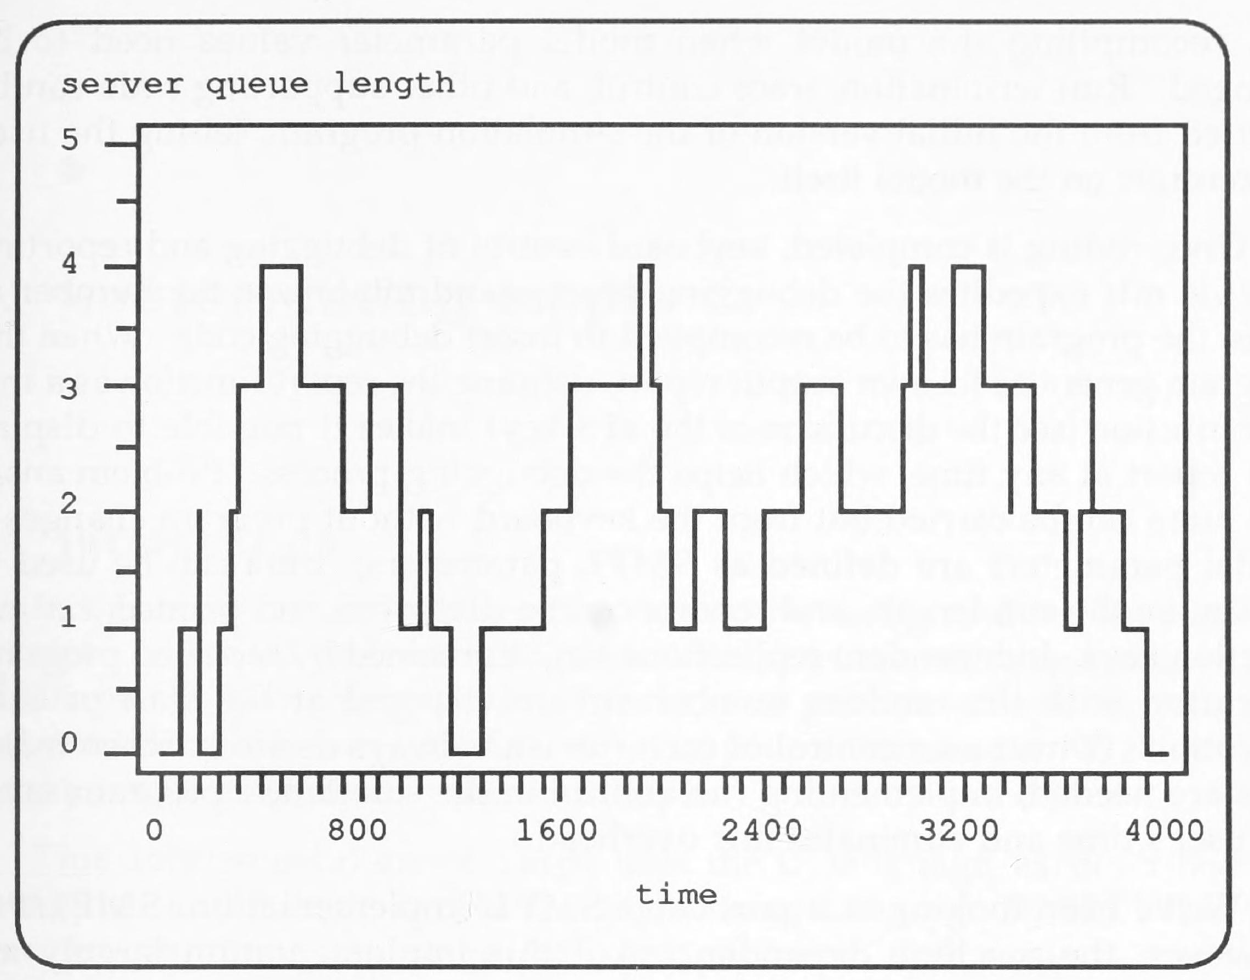
\includegraphics[width=\textwidth]{figures/ch7-figure-7-5.png}
\caption{\texttt{dis} ``step mode'' Plot}
\label{fig:smpl-dis-step}
\end{figure}

\noindent reset key to clear accumulated measures. When the analysis doesn't require
the precision offered by \texttt{bma}, simulation run length can be determined by
plotting the mean value of interest and letting the simulation run until this
value stabilizes. Simply observing the dynamic behavior of a simulated
system is interesting; also, casual observation sometimes reveals bugs that
otherwise might go unnoticed, as evidenced by, for example, unexpected
growth---or lack of growth---of queues.

\section{Summary}
\label{sec:simenv-summary}

The goal of SMPL is to speed the development, testing, and use of small-
and medium-scale simulation models. Defining key input and output
parameters as SMPL parameters reduces implementation time by eliminating
the need to code input processing and report generation functions and, at
the same time, defines potential inputs to the \texttt{table}, \texttt{bma}, and \texttt{dis} modules.
These modules then can be invoked as desired, without coding function calls


\OriginalPage{212}{A Simulation Environment}
\noindent and recompiling the model when model parameter values need to be
changed. Run termination, trace control, and other supporting code can be
omitted from the initial version of the simulation program, letting the user
concentrate on the model itself.

Once coding is completed, keyboard control of debugging and reporting
aids via \texttt{mtr} expedites the debugging process and minimizes the number of
times the program has to be recompiled to insert debugging code. When the
program generates its own output report, defining the report function as a \texttt{mtr}
user function (see the discussion of the sF8 key) makes it possible to display
that report at any time, which helps the debugging process. Problem analysis
often can be carried out from the keyboard without program changes if
model parameters are defined as SMPL parameters; \texttt{bma} can be used to
determine the run length, and reports can be displayed and printed via \texttt{mtr}
function keys. Independent replications can be obtained by repeated program
execution with the random number stream changed at the start of each
execution. (Direct user control of each run isn't always desired; when many
runs are needed, implementing run control in the simulation program saves
the user's time and eliminates \texttt{mtr} overhead.)

We've been looking at a particular SMPL implementation, SMPL/PC.
However, the machine dependencies of this implementation largely are
limited to two areas. There is a screen and keyboard services module (\texttt{svc})
which provides functions for keyboard input and character or graphics screen
output, and \texttt{dis} contains machine-dependent display coordinate mapping
functions. Consequently, transportation of SMPL to other systems should be
straightforward. If you're developing your own simulation system, the key
modules to get in place are \texttt{parms} and \texttt{mtr}; we'll look at the general design of
these and some other SMPL components in Chapter 9.
